\chapter{Integration mit JavaScript}

Im vorherigen Kapitel wurde gezeigt, wie das WebAssembly-Modul (in Form einer \lstinline{wasm}-Datei) erzeugt wird. Grundsätzlich wäre dieses allein theoretisch lauffähig, da aber Interaktion mit JavaScript vorausgesetzt wird (zum Beispiel Objektverwaltung, Konsolenausgaben und native Methoden), ist ein JavaScript-Gerüst rundherum notwendig, das alle Komponenten miteinander verbindet. Daher wird vom Compiler nicht nur ein einfache \lstinline{wasm}-Datei erzeugt, sondern ein Ordner (im Sourcecode \lstinline{Bundle} genannt, nachfolgend auch als "Paket" bezeichnet) mit einigen JavaScript-Dateien und der \lstinline{wasm}-Datei erzeugt.

\section{Aufbau des erzeugten Pakets}

Das Paket hat folgende Ordnerstruktur:
\lstinputlisting{src/javaScriptIntegration/bundleStructure.txt}

Der Name des Wurzelordners ist vom Aufrufer der Compilers frei wählbar, daher wurde er hier als Platzhalter mit \lstinline{<bundle-name>} gekennzeichnet. Alle mit einem \lstinline{(*)} gekennzeichnete Dateien sind von den zu kompilierenden Dateien abhängig und werden dynamisch erzeugt. Alle anderen Dateien sind statisch und sind von den zu kompilierenden Dateien unabhängig. Sie werden 1:1 in den Ordner bei jedem Compileraufruf kopiert.

Nachfolgend einige Details zu den statischen Dateien:

\emph{imports.js} ist für das Erstellen des Import-Objekts verantwortlich, das beim Instanzieren des WebAssembly-Moduls benötigt wird. Hier werden die JavaScript-Implementie\-rungen von sprachinternen Funktionalitäten, als auch die JavaScript-Pendants nativer Methoden in ein Objekt zusammengefasst.

\emph{internal.js} enthält die JavaScript-Implementierungen von sprachinternen Funktionalitäten für Arrays und Stringkonkatenationen.

\emph{runtime.js} definiert die Laufzeitumgebung für das Zusammenspiel zwischen JavaScript und WebAssembly/MiniJavs. Hier befindet sich die Objektverwaltung und diverse Hilfsfunktionen um Daten zwischen JavaScript und WebAssembly/MiniJava auszutauschen und um von JavaScript ausgehend MiniJava-Methoden aufrufen zu können.

Nun zu den dynamischen Dateien:

Alle JavaScript-Pendants für native Methoden werden in den Ordner \emph{native} kopiert. Um dabei potenzielle Dateinamenkollisionen zu umgehen, werden alle Dateien ab 0 beginnend nummeriert.

Der generierte Bytecode wird in der Datei \emph{module.wasm} abgelegt. Als Zwischenprodukt entsteht beim Kompilieren die Datei \emph{module.wat}, die lediglich die textuelle Repräsentation des WebAssembly-Moduls ist, aus dieser Datei entsteht mit dem Werkzeug \lstinline{wat2wasm}\cite{WABT} dann die binäre Form des Moduls. Die textuelle Repräsentation wird zur Laufzeit grundsätzlich nicht benötigt.

Alle im MiniJava-Sourcecode vorhandenen Stringliterale werden in der Datei \emph{module.js} registriert. Außerdem werden zur Compile-Zeit sämtliche Konstrukturen, Getter und Setter für MiniJava-Klassen generiert und in dieser Datei gespeichert. Weiters referenziert diese Datei alle JavaScript-Dateien im \emph{native} Ordner.

Je nachdem, auf welcher Plattform das Paket ausgeführt wird, muss das WebAssembly-Modul unterschiedlich geladen werden: Bei Node.js kann das Module aus dem Dateisystem gelesen werden, im Browser muss es von einem Web-Server heruntergeladen werden. Um dem Benutzer des Pakets  Flexibilität zu ermöglichen, wird das WebAssembly-Modul nicht direkt von den anderen JavaScript-Dateien referenziert.

In der folgenden Grafik wird der Zusammenhang zwischen den JavaScript-Dateien visualisiert:

\begin{center}
    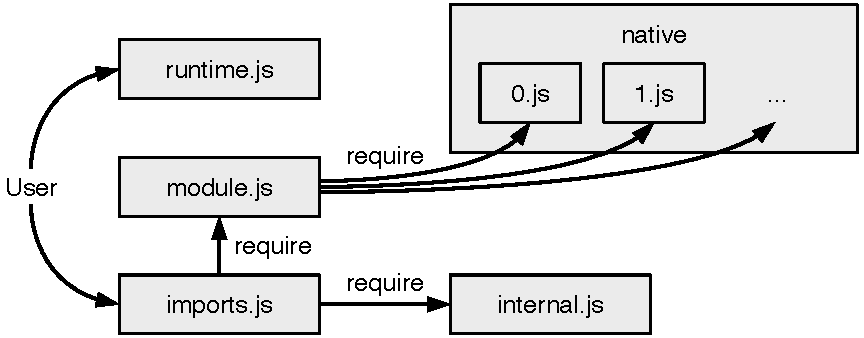
\includegraphics[width=0.8\textwidth]{javaScriptIntegration/bundle}
\end{center}

Auf die praktische Verwendung der JavaScript-Dateien wird in diesem Kapitel nicht eingangen. Im Abschnitt \ref{sec:NodeJSExample} wird anhand eines Beispiels gezeigt, wie sich das Paket in eine Node.js-Konsolenanwendung integrieren lässt.

\section{JavaScript-Codegenerierung}

Wie im vorherigen Abschnitt beschrieben, wird beim Kompilieren JavaScript-Code in der Datei \emph{module.js} generiert.

Beim Erzeugen des Bytecodes wurden bereits für die Stringliterale Speicheradressen (ab 1 beginnend) festgelegt. Daher müssen später zur Laufzeit die Stringliterale in der Reihenfolge der Speicheradressen registriert werden. Dies muss geschehen, bevor das WebAssembly-Modul gestartet wird, da zu diesem Zeitpunkt noch keine Objekte erstellt wurden. So wird garantiert, dass sich die Adressen nicht verschieben.

Außerdem muss für jede Klasse ein Konstruktur generiert werden. Dieser hat die Aufgabe, ein JavaScript-Objekt zu erzeugen, in dem alle Instanzvariablen mit einem (je nach Datentyp) sinnvollen Platzhalterwert initialisiert werden. Außerdem wird der MiniJava-Datentyp mit dem Objekt verknüpft. Die Konstrukturen geben als Rückgabewert die Adresse des erzeugen Objekts zurück.

Da jede Klasse auch Instanzvariablen besitzen kann und WebAssembly nicht direkt auf JavaScript-Objekte zugreifen kann, müssen für diese Getter und Setter erzeugt werden, die diese Aufgabe übernehmen. Die Getter bekommen als Parameter nur die Adresse bzw. Referenz des Objekts und müssen den Wert der Instanzvariable (oder die Adresse wenn die Instanzvariable ein Objekt referenziert) zurückgeben. Ähnlich funktionieren die Setter: Diese bekommen zwei Parameter, die Adresse des Objekts und den Wert des neuen Werts für die Instanzvariable (oder die Adresse, wenn es sich um referenzierte Objekte handelt). Setter haben keinen Rückgabewert.

Die Codegenerierung wird anhand eines überschaubaren Beispiel nun detailliert gezeigt. Nachfolgend sieht man den MiniJava-Code für dieses Beispiel:

\lstinputlisting{src/javaScriptIntegration/Example.minijava}

Aus diesem Code wurde die Datei \emph{module.js} erzeugt:

\lstinputlisting{src/javaScriptIntegration/module.js}

Man sieht am Beginn die zwei Stringliterale (1). Etwas weiter unten ist der Konstruktor, der die Instanzvariablen mit \lstinline{0} und \lstinline{null} initialisiert (2). Bei (3) werden Getter und Setter für die \lstinline{int}-Instanzvariable definiert. Da es sich um einen elementaren Datentyp handelt, kann der Wert direkt aus dem übergebenen Parameter gelesen werden (Setter) bzw. als Rückgabewert zurückgegeben werden (Getter). Beim Getter und Setter für die \lstinline{String}-Instanzvarible (4) muss der Parameter beim Setter zunächst derefenziert werden bzw. muss beim Getter zunächst eine Referenz auf das Objekt erzeugt werden.

\section{Sprachinterne Funktionen}
\subsection{Arrayfunktionen}
\subsection{Stringkonkatenation}

\section{Methodenaufrufe von JavaScript nach MiniJava}

\section{Objektverwaltung für MiniJava in JavaScript}
\subsection{Aufbau}
\subsection{Typinformationen}
\subsection{Hilfsfunktionen}

\section{Auszug aus der Standardbibliothek}
